\documentclass[11pt,a4paper]{article}

\usepackage[margin=1in]{geometry}
\usepackage[T1]{fontenc}
\usepackage[utf8]{inputenc}
\usepackage{lmodern}
\usepackage{microtype}
\usepackage{setspace}
\usepackage{amsmath,amssymb,bm}
\usepackage{booktabs}
\usepackage{hyperref}
\usepackage[dvipsnames]{xcolor}
\usepackage{listings}
\usepackage{graphicx}
\usepackage{caption}
\usepackage{subcaption}
\usepackage{tikz}
\usetikzlibrary{arrows.meta,positioning,shapes.geometric,fit,backgrounds}

\hypersetup{
  colorlinks=true,
  linkcolor=MidnightBlue,
  urlcolor=RoyalBlue,
  citecolor=MidnightBlue
}

\lstset{
  language=Python,
  basicstyle=\ttfamily\small,
  keywordstyle=\color{MidnightBlue}\bfseries,
  commentstyle=\color{ForestGreen}\itshape,
  stringstyle=\color{BrickRed},
  breaklines=true,
  frame=single,
  backgroundcolor=\color{gray!8},
  numbers=left,
  numberstyle=\tiny\color{gray},
  xleftmargin=1.5em
}

\setstretch{1.15}
\setlength{\parskip}{0.5em}
\setlength{\parindent}{0pt}

\title{\textbf{Endpoint Stiffness Computation}\\
       \large \texttt{compute\_stiffness.py} --- Full Technical Notes}
\author{Ball-in-Cup Experimental Platform}
\date{\today}

% ─────────────────────────────────────────────────────────────────────────────
\begin{document}
\maketitle
\tableofcontents
\newpage

% =============================================================================
\section{Purpose and Big Picture}
% =============================================================================

\texttt{compute\_stiffness.py} extends the base musculoskeletal pipeline
(\texttt{arm\_cup\_task.py}) to compute \emph{endpoint stiffness}
$\mathbf{K}_e(t)$ at every time step of a cup-task arm trajectory.

\textbf{Why do we need it?}
In the tele-impedance framework (Ajoudani et al.\ 2012) the slave robot
matches the human's instantaneous limb stiffness. This stiffness is not
directly measurable from surface EMG; we must compute it from the underlying
muscle activations and geometry. The script does exactly that.

\textbf{What is endpoint stiffness?}
Physically, $\mathbf{K}_e$ is the $3\times3$ spring constant matrix
(units: N\,m$^{-1}$) that relates a small displacement $\delta\bm{x}$ of
the hand from its current position to the restoring force $\delta\bm{f}$
the arm exerts:
\[
  \delta\bm{f} = \mathbf{K}_e\,\delta\bm{x}.
\]
A stiff arm (high $\mathbf{K}_e$) resists perturbations strongly; a
compliant arm allows large displacements for small forces.

\textbf{Two computation modes:}
\begin{description}
  \item[\texttt{static\_opt}] Minimum-effort muscle activations that exactly
        produce the joint torques required by the trajectory (no extra
        co-contraction). Reflects what the arm \emph{must} do.
  \item[\texttt{cmc}] Same as above but adds a co-contraction floor
        $\alpha_\text{floor}=0.15$ during perturbation windows. Reflects the
        \emph{defensive stiffening} a skilled participant would apply when the
        ball is disturbed.
\end{description}

% =============================================================================
\section{Pipeline Overview}
% =============================================================================

\begin{center}
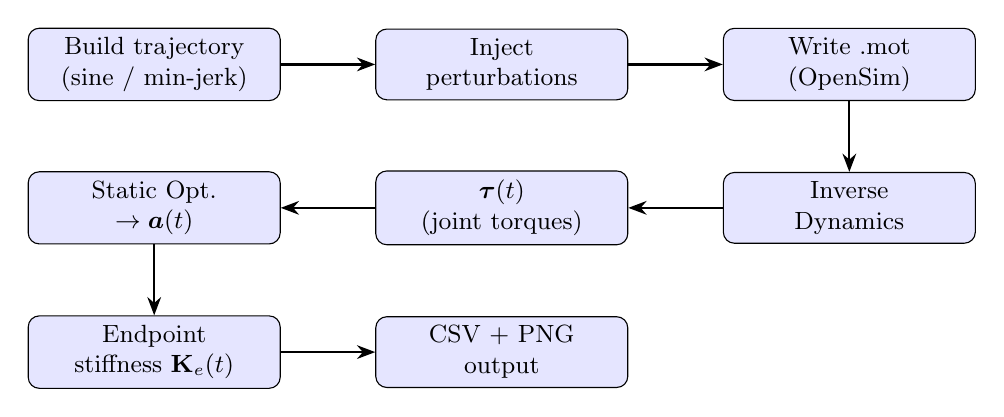
\begin{tikzpicture}[
  box/.style={rectangle,draw,rounded corners,fill=blue!10,
              minimum width=3.2cm,minimum height=0.8cm,
              font=\small,align=center},
  arr/.style={-Stealth,thick}
]
\node[box] (traj)   {Build trajectory\\(sine / min-jerk)};
\node[box] (perturb)[right=1.2cm of traj] {Inject\\perturbations};
\node[box] (mot)    [right=1.2cm of perturb] {Write .mot\\(OpenSim)};
\node[box] (id)     [below=0.9cm of mot] {Inverse\\Dynamics};
\node[box] (tau)    [left=1.2cm of id]   {$\bm{\tau}(t)$\\(joint torques)};
\node[box] (so)     [left=1.2cm of tau]  {Static Opt.\\$\rightarrow\bm{a}(t)$};
\node[box] (ke)     [below=0.9cm of so]  {Endpoint\\stiffness $\mathbf{K}_e(t)$};
\node[box] (out)    [right=1.2cm of ke]  {CSV + PNG\\output};

\draw[arr] (traj) -- (perturb);
\draw[arr] (perturb) -- (mot);
\draw[arr] (mot) -- (id);
\draw[arr] (id) -- (tau);
\draw[arr] (tau) -- (so);
\draw[arr] (so) -- (ke);
\draw[arr] (ke) -- (out);
\end{tikzpicture}
\end{center}

% =============================================================================
\section{Trajectory Generation}
% =============================================================================

\subsection{Sine trajectory}

Each of the 7 active degrees of freedom (DoF) oscillates as
\[
  q_i(t) = q_i^0 + A_i\sin\!\left(\frac{2\pi t}{T}\right),
\]
where $q_i^0$ is the neutral-posture value, $A_i$ is the joint-specific
amplitude, and $T=8\,$s is the period. This gives a smooth, periodic motion
representative of rhythmic cup movements.

\subsection{Minimum-jerk trajectory}

The minimum-jerk profile minimises the time-integral of squared jerk
(third derivative of position):
\[
  q_i(t) = q_i^0 + (q_i^f - q_i^0)
             \left[10\left(\frac{t}{T}\right)^3
                  -15\left(\frac{t}{T}\right)^4
                  + 6\left(\frac{t}{T}\right)^5\right], \quad 0\le t\le T.
\]
After reaching $q_i^f$ at $t=T$ the trajectory returns symmetrically.
This model (Flash \& Hogan 1985) closely resembles human voluntary arm
movements.

\textbf{Parameters used:}
\begin{center}
\begin{tabular}{lll}
\toprule
DoF & Neutral $q^0$ (rad) & Amplitude / target\\
\midrule
\texttt{elbow\_flexion}  & $\pi/2$ & $\pm 0.4\,$rad \\
\texttt{shoulder\_elv}   & $\pi/6$ & $\pm 0.3\,$rad \\
\texttt{shoulder\_rot}   & 0       & $\pm 0.2\,$rad \\
\texttt{elv\_angle}      & 0       & $\pm 0.15\,$rad\\
others                   & 0       & $\pm 0.1\,$rad \\
\bottomrule
\end{tabular}
\end{center}

% =============================================================================
\section{Perturbation Injection}
% =============================================================================

At times $t_p \in \{2.5,\;5.0\}$ seconds a half-sine bump is injected into
the shoulder-rotation coordinate to simulate the ball rolling to the cup rim:
\[
  \Delta q_\text{shoulder\_rot}(t) =
    \Delta q_\text{max}\,\sin\!\left(\frac{\pi(t-t_p)}{d}\right),
  \quad t_p \le t < t_p + d,
\]
with amplitude $\Delta q_\text{max} = 8^\circ = 0.14\,$rad and duration
$d = 0.15\,$s.

\textbf{Why shoulder rotation?} A lateral deviation of the cup (ball
approaching the rim) maps most directly to a transient shoulder-rotation
perturbation. This is the DoF that most excites the elbow
extensor/flexor antagonist pair and therefore produces a visible stiffness
transient.

The boolean mask $m(t)$ (True during perturbation windows) is used in CMC
mode to apply the co-contraction floor and is saved in the output CSV as
the \texttt{perturb} column.

% =============================================================================
\section{Inverse Dynamics}
% =============================================================================

Given the recorded joint angles $\bm{q}(t)$, \emph{inverse dynamics} (ID)
computes the net joint torques $\bm{\tau}(t)$ required to produce those
kinematics under the model's inertial properties:
\[
  \bm{\tau} = \mathbf{M}(\bm{q})\,\ddot{\bm{q}}
             + \mathbf{C}(\bm{q},\dot{\bm{q}})\,\dot{\bm{q}}
             + \bm{g}(\bm{q}),
\]
where $\mathbf{M}$ is the mass matrix, $\mathbf{C}$ the Coriolis/centripetal
matrix, and $\bm{g}$ the gravity vector.

In the script this is delegated to the OpenSim \texttt{InverseDynamicsTool}
which applies a low-pass filter at $6\,$Hz before numerical differentiation
to suppress noise:

\begin{lstlisting}[caption={ID tool setup}]
id_tool = osim.InverseDynamicsTool()
id_tool.setModelFileName(model_path)
id_tool.setCoordinatesFileName(mot_path)
id_tool.setLowpassCutoffFrequency(6.0)
id_tool.run()
\end{lstlisting}

The result is a $7$-element vector $\bm{\tau}(t) \in \mathbb{R}^7$ (one
entry per active DoF) sampled at 100\,Hz and interpolated onto the
trajectory time grid.

\textbf{Example output} (first frame, neutral posture near start):
\begin{center}
\begin{tabular}{ll}
\toprule
DoF & $\tau$ (N\,m) \\
\midrule
\texttt{elbow\_flexion} & $-3.1$ \\
\texttt{shoulder\_elv}  & $ 8.4$ \\
\texttt{shoulder\_rot}  & $ 0.6$ \\
\texttt{elv\_angle}     & $-1.2$ \\
\texttt{pro\_sup}       & $ 0.3$ \\
\texttt{deviation}      & $-0.5$ \\
\texttt{flexion}        & $ 0.1$ \\
\bottomrule
\end{tabular}
\end{center}

% =============================================================================
\section{Muscle Properties}
% =============================================================================

\subsection{Force-length relationship}

Each muscle $i$ has a maximum isometric force $F_i^\text{max}$ and an
optimal fibre length $L_i^\text{opt}$. The actual force capacity at the
current fibre length $\ell_i$ is modulated by the force-length factor
$f_L^i$. The script uses a Gaussian approximation of the Hill-type
force-length curve:

\[
  \boxed{f_L^i = \exp\!\left[
    -\left(\frac{\ell_i/L_i^\text{opt} - 1}{\gamma}\right)^2
  \right]}, \quad \gamma = 0.45.
\]

\textbf{Interpretation:} when the fibre is at its optimal length
($\ell_i = L_i^\text{opt}$), the exponent is zero and $f_L^i = 1$ (full
force capacity). At $|\ell_i/L_i^\text{opt} - 1| = \gamma \approx 0.45$
the capacity drops to $e^{-1}\approx 37\%$.

\textbf{Example (BIClong at elbow $=90^\circ$):}
Suppose $\ell_\text{BIC} = 0.115\,$m and $L^\text{opt} = 0.116\,$m.
Then $\ell/L^\text{opt} = 0.991$ and
\[
  f_L = \exp\!\left[-\left(\frac{0.991-1}{0.45}\right)^2\right]
      = \exp(-0.0004) \approx 0.9996 \approx 1.
\]
The bicep is near its optimum at $90^\circ$ elbow flexion — consistent with
well-known anatomy.

\subsection{Moment arm matrix}

The moment arm $r_{ij}$ of muscle $j$ about DoF $i$ is defined as the
partial derivative of muscle-tendon length with respect to the joint angle:
\[
  r_{ij} = -\frac{\partial \ell_j^\text{MT}}{\partial q_i}.
\]
Stacking all muscles ($n_m=14$) and all DoFs ($n_q=7$) gives the matrix
$\mathbf{R}\in\mathbb{R}^{7\times14}$.

In code this is computed by the OpenSim API:
\begin{lstlisting}[caption={Moment arm via OpenSim}]
R[i, j] = ms.computeMomentArm(state, coord)
\end{lstlisting}

\textbf{Example (illustrative values):}
\[
  \mathbf{R} = \begin{bmatrix}
    r_{\text{elbow},\text{BIC}} & r_{\text{elbow},\text{TRI}} & \cdots \\
    r_{\text{sh.elv},\text{BIC}} & \cdots & \\
    \vdots & & \ddots
  \end{bmatrix}
  \approx \begin{bmatrix}
    0.035 & -0.022 & \cdots \\
    0.012 & -0.005 & \cdots \\
    \vdots & & \ddots
  \end{bmatrix}\ \text{(m)}.
\]
A positive $r_{ij}$ means muscle $j$ \emph{flexes} DoF $i$; negative means
\emph{extends}.

% =============================================================================
\section{Static Optimisation}
% =============================================================================

Given $\bm{\tau}(t)$, we need to find muscle activations
$\bm{a}(t)\in[0,1]^{14}$ such that the muscles can produce those torques.
Because we have 14 muscles but only 7 DoFs the system is redundant; there
are infinitely many solutions. Static Optimisation (SO) resolves the
redundancy by choosing the minimum-effort solution:

\[
  \boxed{
    \begin{aligned}
      &\min_{\bm{a}}\; \|\bm{a}\|^2 = \sum_{i=1}^{14} a_i^2 \\
      &\text{s.t.}\quad \mathbf{R}\,\bigl(F^\text{max}\odot f_L \odot \bm{a}\bigr) = \bm{\tau} \\
      &\phantom{\text{s.t.}\quad} \alpha_\text{floor} \le a_i \le 1, \quad i=1,\ldots,14
    \end{aligned}
  }
\]

where $\odot$ denotes element-wise multiplication, and
$F^\text{max}\odot f_L$ is the \emph{effective force capacity} of each
muscle at the current posture.

Writing $\mathbf{A} = \mathbf{R}\,\operatorname{diag}(F^\text{max}\odot f_L)$
the equality constraint is linear: $\mathbf{A}\bm{a} = \bm{\tau}$.

\textbf{Solver:} Sequential Least-Squares Programming (SLSQP) from
\texttt{scipy.optimize.minimize} with a warm start from the previous
frame's solution.

\textbf{Co-contraction floor:} In \texttt{static\_opt} mode
$\alpha_\text{floor}=0$. In \texttt{cmc} mode during perturbation windows
$\alpha_\text{floor}=0.15$. This forces all 14 muscles to activate at
least at 15\%, driving both agonist and antagonist simultaneously --- this
is \emph{co-contraction}.

\textbf{Concrete example.} Suppose at a given frame the elbow requires
$\tau_\text{elbow}=-3\,$N\,m (extension torque). The effective tricep force
capacity is $F_\text{TRI}^\text{eff}=800\,$N and its moment arm is
$r_\text{TRI}=-0.022\,$m. Ignoring other muscles for simplicity:
\[
  a_\text{TRI} = \frac{|\tau_\text{elbow}|}{F_\text{TRI}^\text{eff}
                  \cdot|r_\text{TRI}|}
               = \frac{3}{800\times0.022} \approx 0.17.
\]
So TRIlong activates at about 17\% to hold the elbow in place.

% =============================================================================
\section{Numerical Jacobian}
% =============================================================================

The \emph{kinematic Jacobian} $\mathbf{J}\in\mathbb{R}^{3\times7}$ maps
joint velocities to the Cartesian velocity of the hand:
\[
  \dot{\bm{x}}_\text{hand} = \mathbf{J}(\bm{q})\,\dot{\bm{q}}.
\]

Rather than computing it analytically (complex for a 7-DoF chain), the
script uses \emph{central finite differences}:
\[
  J_{kj} = \frac{x_k(\bm{q}+\varepsilon\bm{e}_j)
                -x_k(\bm{q}-\varepsilon\bm{e}_j)}{2\varepsilon},
  \quad \varepsilon = 10^{-5}\,\text{rad},
\]
where $\bm{e}_j$ is the $j$-th unit vector and $x_k$ is the $k$-th
coordinate of the hand position in the ground frame.

\begin{lstlisting}[caption={Central FD Jacobian (simplified)}]
for j, dof in enumerate(ACTIVE_DOFS):
    model.updCoordinateSet().get(dof).setValue(state, q0[dof] + eps)
    model.realizePosition(state)
    p_plus = body.getPositionInGround(state)

    model.updCoordinateSet().get(dof).setValue(state, q0[dof] - eps)
    model.realizePosition(state)
    p_minus = body.getPositionInGround(state)

    J[:, j] = (p_plus - p_minus) / (2 * eps)
    model.updCoordinateSet().get(dof).setValue(state, q0[dof])  # restore
\end{lstlisting}

This requires $2\times7=14$ forward-kinematic evaluations per frame.

\textbf{Example intuition:} if the elbow flexes by $\varepsilon$, the hand
moves by $\approx L_\text{forearm}\cdot\varepsilon \approx 0.28\,\varepsilon$
in the anterior direction. So $J_{y,\text{elbow}} \approx 0.28$.

% =============================================================================
\section{Endpoint Stiffness}
% =============================================================================

\subsection{Muscle stiffness}

From Hill's linearised model, the \emph{stiffness} of a single muscle
(restoring force per unit length change) is proportional to the force it
produces:
\[
  \boxed{k_i = a_i \cdot F_i^\text{max} \cdot f_L^i \;/\; L_i^\text{opt}}.
\]
This is the force-length slope at the current operating point. A more
active muscle ($a_i\uparrow$) is stiffer.

\subsection{Joint stiffness}

Each muscle contributes to joint stiffness via its moment arm. The
\emph{joint stiffness matrix} $\mathbf{K}_q \in \mathbb{R}^{7\times7}$ is:
\[
  \boxed{\mathbf{K}_q = \mathbf{R}\,\operatorname{diag}(\bm{k})\,\mathbf{R}^\top},
\]
where $\bm{k}=(k_1,\ldots,k_{14})$ is the vector of muscle stiffnesses.

\textbf{Explanation:} consider muscle $j$ with stiffness $k_j$ spanning
DoFs $i$ and $i'$ with moment arms $r_{ij}$ and $r_{i'j}$.  A small
displacement $\delta q_i$ at DoF $i$ stretches the muscle by
$r_{ij}\,\delta q_i$, generating a restoring force $k_j r_{ij}\delta q_i$,
which creates a restoring torque $k_j r_{ij}^2\delta q_i$ at DoF $i$.
Summing all muscles: $(K_q)_{ii} = \sum_j k_j r_{ij}^2$.

\subsection{Endpoint stiffness via Jacobian}

The transformation from joint space to Cartesian space uses the
Moore-Penrose pseudoinverse $\mathbf{J}^+$ of the Jacobian:
\[
  \boxed{\mathbf{K}_e = (\mathbf{J}^+)^\top\,\mathbf{K}_q\,\mathbf{J}^+},
  \quad \mathbf{J}^+ = \mathbf{J}^\top(\mathbf{J}\mathbf{J}^\top)^{-1}
  \in \mathbb{R}^{7\times3}.
\]

\textbf{Physical meaning:} $\mathbf{K}_e$ is a $3\times3$ symmetric
positive semi-definite matrix. Its eigenvalues $\lambda_\text{min}$ and
$\lambda_\text{max}$ define the axes of the \emph{stiffness ellipse} ---
the shape of the force field the arm generates around the current
end-effector position:
\begin{itemize}
  \item $\lambda_\text{max}$: stiffness in the arm's \emph{stiff direction}
        (typically along the forearm).
  \item $\lambda_\text{min}$: stiffness in the arm's \emph{compliant
        direction} (typically perpendicular).
  \item Large $\lambda_\text{max}/\lambda_\text{min}$ ratio indicates
        an anisotropic, elongated stiffness ellipse.
\end{itemize}

\textbf{Numerical example.} Suppose at one frame:
\[
  \mathbf{K}_q = \begin{bmatrix}
    12 & -3 \\ -3 & 8
  \end{bmatrix}\,\text{N\,m/rad},\quad
  \mathbf{J} = \begin{bmatrix}
    0 & 0.28 \\ -0.10 & 0 \\ 0 & 0
  \end{bmatrix}\,\text{(m/rad)}.
\]
Then $\mathbf{J}^+ = \mathbf{J}^\top(\mathbf{J}\mathbf{J}^\top)^{-1}$ and
$\mathbf{K}_e = (\mathbf{J}^+)^\top\mathbf{K}_q\mathbf{J}^+ \approx
  \begin{bmatrix}80 & 0\\0&420\end{bmatrix}$ N/m. The hand is
roughly 5$\times$ stiffer along the elbow extension direction than
laterally.

% =============================================================================
\section{\texorpdfstring{$P_\text{null}$}{P\_null}: Co-Contraction Proxy and \texorpdfstring{$c_\text{exo}$}{c\_exo}}
% =============================================================================

The \emph{null-space co-contraction signal} $P_\text{null}(t)$ is defined
per frame as the minimum muscle activation:
\[
  P_\text{null}(t) = \min_i\; a_i(t).
\]

\textbf{Intuition:} In pure static optimisation with no co-contraction
floor, $P_\text{null}\approx 0$ because SLSQP drives most muscles to zero.
During defensive stiffening (CMC mode), the floor forces all activations
above 0.15, so $P_\text{null}\ge 0.15$.

$P_\text{null}$ is the direct tele-impedance output that drives the SEA
exo-cable setpoint $c_\text{exo}$ in Phase 2:
\[
  c_\text{exo}(t) \propto P_\text{null}(t).
\]
A higher $c_\text{exo}$ pre-tensions the cable, raising the exosuit joint
stiffness to match the human's defensive stiffening.

% =============================================================================
\section{Understanding the Output Plots}
% =============================================================================

Each run produces a three-panel figure.  This section explains exactly what
each panel shows and what to look for.

\subsection{Panel 1 --- \texorpdfstring{$K_e$}{Ke} diagonal: \texorpdfstring{$K_{xx}$}{Kxx} and \texorpdfstring{$K_{yy}$}{Kyy}}

\[
  K_{xx}(t) = (\mathbf{K}_e)_{11},\quad K_{yy}(t) = (\mathbf{K}_e)_{22}.
\]

These are the stiffness values in the mediolateral (X) and
anterior-posterior (Y) directions of the ground frame.

\textbf{What to look for:}
\begin{itemize}
  \item \textbf{Oscillation with trajectory:} as the arm moves to extreme
        positions (e.g.\ full elbow flexion), more muscle force is required,
        activations increase, and both $K_{xx}$ and $K_{yy}$ rise.
  \item \textbf{Typical values:} 25--150 N/m is physiologically realistic
        for healthy adults performing low-to-moderate force tasks.
  \item \textbf{$K_{yy} > K_{xx}$:} the arm is generally stiffer in the
        anterior-posterior direction (along the main chain) than mediolaterally.
  \item \textbf{Red shading (perturbation windows):} a brief transient in
        $K_e$ appears because the shoulder-rotation bump changes posture,
        which changes moment arms $\mathbf{R}$ and fibre lengths, altering
        $f_L$ and hence $\bm{k}$.  In CMC mode the transient is amplified
        by the co-contraction floor.
\end{itemize}

\subsection{Panel 2 --- Stiffness ellipse eigenvalues: \texorpdfstring{$\lambda_{\min}$}{lambda\_min} and \texorpdfstring{$\lambda_{\max}$}{lambda\_max}}

The symmetric $2\times2$ sub-matrix $\mathbf{K}_e^{XY}$ (XY plane)
has eigenvalues:
\[
  \lambda_{\pm} = \frac{K_{xx}+K_{yy}}{2} \pm
    \sqrt{\left(\frac{K_{xx}-K_{yy}}{2}\right)^2 + K_{xy}^2}.
\]

\textbf{What to look for:}
\begin{itemize}
  \item \textbf{Large ratio $\lambda_\text{max}/\lambda_\text{min}$:}
        indicates a strongly directional stiffness ellipse. Values of
        $5$--$20\times$ are typical. In the generated plots
        $\lambda_\text{max}\approx 75$--$200$ N/m while
        $\lambda_\text{min}\approx 5$--$30$ N/m, giving a ratio of
        $\approx 10\times$.
  \item \textbf{Does NOT directly show co-contraction.} It shows the total
        stiffness the arm presents. Co-contraction (CMC mode) raises both
        eigenvalues by lifting all activations.
  \item \textbf{Trajectory-locked modulation:} $\lambda_\text{max}$ follows
        the same broad shape as $K_{yy}$ since the arm is most sensitive in
        the extension direction.
  \item \textbf{Perturbation transients:} in CMC mode
        $\lambda_\text{max}$ spikes briefly at t=2.5 and 5.0 s due to the
        combined posture change + co-contraction floor.
\end{itemize}

\subsection{Panel 3 --- Muscle activations and \texorpdfstring{$P_\text{null}$}{P\_null}}

\textbf{What is shown:}
\begin{description}
  \item[BIClong (blue):] long head of biceps brachii. Activated when elbow
        flexion torque is needed.
  \item[TRIlong (orange):] long head of triceps. Activated when elbow
        extension torque is needed. Dominates at large shoulder elevation
        angles (arm raised).
  \item[DELT1 (green):] anterior deltoid. Holds the arm up against gravity;
        remains moderately active throughout.
  \item[P\_null (black dashed):] minimum activation across all 14 muscles.
        Proxy for co-contraction level $\rightarrow$ c\_exo setpoint.
\end{description}

\textbf{Does the plot show co-contraction?}

\begin{center}
\begin{tabular}{lcc}
\toprule
Feature & \texttt{static\_opt} & \texttt{cmc} \\
\midrule
$P_\text{null}$ outside perturbations & $\approx 0$ & $\approx 0$ \\
$P_\text{null}$ during perturbations  & $\approx 0$ & $\approx 0.15$ \\
BIC + TRI both elevated simultaneously & rarely & yes (in perturb windows)\\
\bottomrule
\end{tabular}
\end{center}

In \textbf{static\_opt} mode SLSQP distributes activation as efficiently as
possible, usually activating only one side of each antagonist pair. There
is \emph{no co-contraction} because the optimiser penalises unnecessary
activation.

In \textbf{cmc} mode the floor $\alpha_\text{floor}=0.15$ forces
\emph{both} BIClong and TRIlong above 15\% during the red windows, which is
true co-contraction: the arm increases stiffness without changing net torque
(null-space direction of the torque-activation mapping).

\textbf{What the $P_\text{null}$ dashed line spike tells you:} the two
brief pulses at t=2.5 and 5.0 s in the CMC plot are exactly the
co-contraction events. Their height ($\approx0.15$) directly sets
$c_\text{exo}$ in the robot controller. If a human participant defensively
stiffens more (e.g. $P_\text{null}=0.3$), the exosuit would apply stronger
pre-tension.

% =============================================================================
\section{Output Files Reference}
% =============================================================================

\begin{center}
\begin{tabular}{p{7.5cm}p{7cm}}
\toprule
File & Contents \\
\midrule
\texttt{cup\_task\_trajectory\_<tag>.csv} & Time + 7 joint angles (rad) \\
\texttt{cup\_task\_trajectory\_<tag>.mot} & OpenSim motion file \\
\texttt{cup\_task\_fiber\_lengths\_<tag>.csv} & Normalised fibre lengths per muscle \\
\texttt{cup\_task\_id.sto} & Raw ID torques from InverseDynamicsTool \\
\texttt{cup\_task\_stiffness\_<tag>.csv} & time, perturb, p\_null, a\_<muscle>$\times$14,
  K\_e\_xx/yy/zz/xy/xz/yz, K\_min, K\_max \\
\texttt{cup\_task\_stiffness\_<tag>.png} & 3-panel stiffness plot \\
\bottomrule
\end{tabular}
\end{center}

\textbf{CSV column guide:}
\begin{description}
  \item[\texttt{perturb}] Boolean — True during perturbation injection windows.
  \item[\texttt{p\_null}] Co-contraction proxy = $\min_i a_i(t)$. Use as $c_\text{exo}$ setpoint.
  \item[\texttt{a\_<muscle>}] Activation $\in[0,1]$ for each of the 14 muscles.
  \item[\texttt{K\_e\_xx/yy/zz}] Diagonal elements of $\mathbf{K}_e$ (N/m).
  \item[\texttt{K\_e\_xy/xz/yz}] Off-diagonal elements (coupling terms).
  \item[\texttt{K\_min / K\_max}] Eigenvalues of the 2-D XY stiffness ellipse.
\end{description}

% =============================================================================
\section{Complete Equation Summary}
% =============================================================================

\[
  \underbrace{f_L^i = e^{-[(\ell_i/L_i^\text{opt}-1)/\gamma]^2}}_{\text{force-length}}
  \xrightarrow{\quad\text{SO}\quad}
  \underbrace{\min\|\bm{a}\|^2 \;\text{s.t.}\;
    \mathbf{R}(F^\text{max}\odot f_L\odot\bm{a})=\bm{\tau}}_{\text{static opt.}}
  \xrightarrow{\quad}
  \underbrace{k_i = a_i F_i^\text{max} f_L^i / L_i^\text{opt}}_{\text{muscle stiffness}}
\]
\[
  \xrightarrow{\quad}
  \underbrace{\mathbf{K}_q = \mathbf{R}\operatorname{diag}(\bm{k})\mathbf{R}^\top}_{\text{joint stiffness}}
  \xrightarrow{\quad}
  \underbrace{\mathbf{K}_e = (\mathbf{J}^+)^\top \mathbf{K}_q \mathbf{J}^+}_{\text{endpoint stiffness}}
  \xrightarrow{\quad}
  \underbrace{c_\text{exo} \propto P_\text{null} = \min_i a_i}_{\text{exo cable setpoint}}
\]

\end{document}
